\documentclass[12pt,a4paper]{article}

% ─── Packages ─────────────────────────────────────────────────
\usepackage[utf8]{inputenc}
\usepackage[T1]{fontenc}
\usepackage{geometry}
\usepackage{titlesec}
\usepackage{enumitem}
\usepackage{graphicx}
\usepackage{xcolor}
\usepackage{hyperref}
\usepackage{booktabs}
\usepackage{array}
\usepackage{longtable}
\usepackage{parskip}
\usepackage{fancyhdr}
\usepackage{lastpage}

% ─── Page geometry ────────────────────────────────────────────
\geometry{margin=2.5cm}
\pagestyle{fancy}
\fancyhf{}
\fancyhead[L]{\small CSC2106 --- Real-Time File Transfer System using CoAP}
\fancyhead[R]{\small BugattiFerrariLamborghini}
\fancyfoot[C]{\thepage\ of \pageref{LastPage}}

% ─── Section formatting ──────────────────────────────────────
\titleformat{\section}{\large\bfseries}{Section \Roman{section}: }{0em}{}
\titleformat{\subsection}{\normalsize\bfseries}{\thesubsection}{1em}{}

% ─── Hyperref ─────────────────────────────────────────────────
\hypersetup{
    colorlinks=true,
    linkcolor=blue,
    citecolor=blue,
    urlcolor=blue
}

% ─── Custom commands ──────────────────────────────────────────
\DeclareRobustCommand{\changed}[1]{#1}
\DeclareRobustCommand{\forecast}[1]{\textbf{[Forecasted]} #1}

\begin{document}

% ═════════════════════════════════════════════════════════════
% TITLE PAGE
% ═════════════════════════════════════════════════════════════

\begin{center}
    \vspace*{1cm}
    {\Large \textbf{Project: [CSC2106] Real-Time File Transfer System using CoAP}} \\[0.5cm]
    {\large Date: 18 March 2026} \\[0.3cm]
    {\large Team Name: BugattiFerrariLamborghini} \\[1cm]

    \begin{tabular}{|p{7cm}|p{4cm}|}
        \hline
        \textbf{Student Name} & \textbf{Student ID} \\
        \hline
        Pang Jia De & 2402226 \\
        \hline
        Dui Rui En Joshua & 2402201 \\
        \hline
        Tan Jian Xin & 2401421 \\
        \hline
        Tan Bing Kun Terence & 2401883 \\
        \hline
    \end{tabular}

    \vspace{0.8cm}
    \changed{\textbf{Source Code Repository:} \url{https://github.com/Daddycation23/IOTForestCam}}
\end{center}

\vspace{1.5cm}

% ═════════════════════════════════════════════════════════════
% ABSTRACT
% ═════════════════════════════════════════════════════════════

\section*{Abstract}
% (150--250 words)

\changed{Selecting an appropriate communications technology for off-grid forest wildlife monitoring requires balancing range, throughput, and idle power simultaneously, a three-way trade-off that no single radio stack resolves. This project frames the problem as a technology-selection exercise: surveying seven candidate wireless technologies (LoRa 2.4\,GHz, LoRaWAN, Wi-Fi, BLE, Zigbee, LTE-M/NB-IoT, and Sigfox) against the constraints of battery-only operation, absence of cellular infrastructure, multi-megabyte image payloads, and multi-hop coordination, then building and validating a prototype around the only combination that satisfies all five hard constraints.}
The resulting system is a Hybrid IoT Mesh Network built on ESP32-S3 microcontrollers with LILYGO T3-S3 V1.2 boards featuring the SX1280 2.4\,GHz LoRa transceiver. The proposed architecture decouples the control and data planes: a LoRa radio module serves exclusively as a low-power control plane, while sensor nodes utilize timer-based deep sleep ($<$10\,$\mu$A) with 180-second wake intervals to minimize idle power consumption. \changed{The gateway node runs a persistent Wi-Fi access point. Leaf nodes connect as station (STA) clients on timer wake, announce their presence via CoAP POST, and serve images for download.} High-bandwidth payloads, simulated in this prototype via pre-loaded images on SD cards, are segmented and \changed{reliably} transmitted \changed{over the Wi-Fi data plane} using CoAP block-wise transfer over UDP. \changed{The system employs FreeRTOS dual-core task separation to eliminate LoRa blackouts during harvest, AODV reactive mesh routing for multi-hop coordination, a Bully election algorithm for automatic gateway selection, and automatic role negotiation so nodes self-organize without manual configuration.} By shifting from a continuous-listening network to an event-driven hybrid model, this system drastically minimizes idle power consumption while retaining the capacity to route large files across multiple hops. The resulting prototype demonstrates a scalable, energy-efficient framework capable of delivering real-time visual alerts to a local gateway, shifting remote forest monitoring from reactive manual data retrieval to proactive, real-time intervention.

\newpage

% ═════════════════════════════════════════════════════════════
% SECTION I: INTRODUCTION, PROBLEM STATEMENT AND OBJECTIVES
% ═════════════════════════════════════════════════════════════

\section{Introduction, Problem Statement and Objectives}
% (Word Limit: 750 words)

\subsection{Introduction}

Effective environmental monitoring and forest conservation is critical for biodiversity preservation and disaster mitigation, which require sensor networks capable of operating autonomously in remote, off-grid environments. Currently, the industry relies heavily on manual data retrieval from local storage, which is a labor-intensive and reactive approach. This project proposes a Hybrid IoT Mesh Network utilizing ESP32-S3 microcontrollers to bridge the gap between remote sensing and real-time data access. By integrating LoRa for long-range, low-power control signaling and Wi-Fi for high-bandwidth data transfer, the system offers a highly scalable solution. \changed{To ensure rigorous and deterministic validation of the underlying network routing, this iteration of the project replaces live camera hardware with an SD card containing pre-loaded images. This approach utilizes images with various resolutions pre-loaded onto SD cards, eliminating camera hardware-induced errors and isolating the network's performance metrics for more accurate testing.} The system employs periodic wake cycles combined with event-driven coordination, enabling all high-bandwidth communications to utilize CoAP over UDP for lightweight, reliable image transmission via block-wise transfer. This architecture shifts remote monitoring from reactive data retrieval to proactive intervention.

\subsection{Problem Statement}

The primary challenge in off-grid environmental monitoring is the ``Data Latency Gap.'' Standard methods store data locally on SD cards, resulting in weeks or months of delay between an event occurring and its detection. While real-time wireless alternatives exist, they face a strict ``Bandwidth-Range-Power Trilemma'': low-power wide-area technologies (like LoRa) lack the bandwidth required for image transfer, while high-bandwidth solutions (like standard Wi-Fi or cellular networks) consume excessive energy and lack coverage in deep forests.

This project directly addresses this gap by decoupling the control and data transport layers, solving the power constraints that traditionally limit the long-term deployment of visual sensors. \changed{Furthermore, traditional embedded vision nodes frequently suffer from heap memory exhaustion when processing large image buffers in real-time. By implementing a storage-driven data pipeline that streams data directly from an SD card to the Wi-Fi buffer in 1024-byte chunks, this project circumvents the RAM limitations of the ESP32-S3. Additionally, the network design has been improved to operate completely independently of commercial LoRaWAN or 4G infrastructure; the gateway is now implemented purely as a designated ``Root Node'' within the network, bridging directly to a local diagnostic server for highly localized, off-grid deployment.}

\subsection{Objectives}

The main goal of this project is to develop and validate a functional prototype of a hybrid sensor node that overcomes the limitations of single-protocol networks. The specific objectives are categorized into implemented features and future work:

\subsubsection{Implemented Objectives}

\begin{enumerate}
    \item \textbf{Design a Hybrid Network Architecture:} Develop a sensor node utilizing the ESP32-S3 that integrates both LoRa \changed{(SX1280)} and Wi-Fi radios to optimize the trade-off between transmission range and data bandwidth.

    \item \textbf{Implement Low-Power Sleep Management:} Engineer a highly efficient power management system using timer-based deep sleep ($<$10\,$\mu$A) with 180-second wake intervals. \changed{Note: The originally planned LoRa DIO1 hardware interrupt wake mechanism is non-functional on the LILYGO T3-S3 V1.2 hardware; timer-based wake serves as the primary implementation.}

    \item \textbf{Optimize Image Transfer:} Implement CoAP over UDP with Block-Wise Transfer mechanisms to enable the reliable transmission of large payloads over a lossy, multi-hop Wi-Fi mesh.

    \item \textbf{Develop Dynamic Role Assignment:} Implement a flexible role configuration system allowing all ESP32-S3 nodes to be assigned as Leaf, Relay, or Gateway at deployment, with persistence across power cycles. \changed{Extend this with automatic role negotiation via a Bully election algorithm, enabling nodes to self-organize without manual configuration.}

    \item \changed{\textbf{Develop a File Reading Pipeline:} Design an SD-card-based file I/O system that simulates physical camera captures by randomly reading and segmenting pre-loaded JPEG files into network-safe chunks, ensuring stable payload generation without memory allocation failures.}

    \item \textbf{Evaluate System Performance:} Quantitatively assess the prototype against standard engineering metrics, specifically measuring idle power consumption, total network throughput, and successful multi-hop packet delivery rates in a simulated deployment environment.
\end{enumerate}

\subsubsection{Future Work}

The following objectives remain as planned enhancements beyond the current implementation scope:

\begin{enumerate}
    \item \textbf{Implement Queue-Based Scheduling:} Design a gateway-managed transmission queue that assigns time-division slots to prevent network congestion, ensuring only one node transmits image data at a time. \changed{Current implementation uses sequential harvest without explicit time-slot allocation.}

    \item \textbf{Security and Encryption:} Implement AES-128 encryption for LoRa control-plane packets to protect against eavesdropping and tampering. \changed{Current implementation transmits all packets in cleartext.}
\end{enumerate}

\newpage

% ═════════════════════════════════════════════════════════════
% SECTION II: LITERATURE REVIEW
% ═════════════════════════════════════════════════════════════

\section{Literature Review}
\label{sec:lit-review}

\subsection{Current State of Knowledge and Technology}

The current state of environmental monitoring is transitioning from offline, manual camera traps to connected Wireless Sensor Networks (WSNs) [1]. However, existing deployments remain highly fragmented based on radio capabilities. High-bandwidth networks generally rely on 4G/LTE or standard Wi-Fi, which lack coverage in remote forests and require substantial power infrastructure [2]. Conversely, Low-Power Wide-Area Networks (LPWANs) like LoRa provide excellent multi-kilometer range (2--10\,km line-of-sight) and run on small batteries with idle current $<$20\,$\mu$A, but are strictly limited to low-byte telemetry with maximum payload sizes of 222 bytes per packet and effective throughput $<$5\,kbps due to duty cycle restrictions [3].

\subsection{Candidate Communications Technologies}

\changed{No single wireless technology simultaneously provides long range, high throughput, low idle power, and licence-free operation. Table~\ref{tab:comms-tech} summarises the seven candidate technologies that were considered for this project, drawn from the LPWAN and short-range WSN literature [2]--[4], [11], [12]. The table compares each candidate against the five properties that matter for an off-grid forest camera: maximum range in line-of-sight conditions, effective application-layer throughput, idle current draw, maximum practical payload per packet, licence regime, and whether the technology requires external infrastructure (gateways, carriers, or network servers) to function.}

\begin{table}[ht]
\centering
\small
\caption{Comparison of candidate communications technologies.}
\label{tab:comms-tech}
\begin{tabular}{@{}lrrrrll@{}}
\toprule
\textbf{Technology} & \textbf{Range} & \textbf{Throughput} & \textbf{Idle} & \textbf{Payload} & \textbf{Band} & \textbf{Infra.} \\
\midrule
LoRa 2.4\,GHz (SX1280) [9]  & 2--10\,km & 0.5--202\,kbps   & $<$20\,$\mu$A  & 255\,B  & ISM 2.4\,GHz      & None (P2P/mesh) \\
LoRaWAN sub-GHz [3]         & 2--15\,km & $<$5\,kbps       & $<$20\,$\mu$A  & 222\,B  & ISM sub-GHz       & LoRaWAN gw+NS   \\
Wi-Fi 802.11 (ESP32) [2]    & 50--100\,m & 10--150\,Mbps   & 80--200\,mA    & 1500\,B & ISM 2.4/5\,GHz    & Access point    \\
BLE 5.x [12]                & 30--100\,m & 1--2\,Mbps      & 10--40\,$\mu$A & 247\,B  & ISM 2.4\,GHz      & None (P2P/mesh) \\
Zigbee / 802.15.4 [11]      & 10--100\,m & 250\,kbps       & 20--50\,$\mu$A & 127\,B  & ISM 2.4\,GHz      & Coordinator     \\
LTE-M / NB-IoT              & Cellular   & 0.2--1\,Mbps    & 100--200\,mA*  & 1500\,B & Licensed cellular & Carrier/SIM     \\
Sigfox                      & 10--40\,km & 0.1\,kbps       & $<$20\,$\mu$A  & 12\,B   & ISM sub-GHz       & Sigfox network  \\
\bottomrule
\end{tabular}

\vspace{0.3em}
{\footnotesize *Transmit current; PSM idle can be lower but requires carrier PSM support and still draws $>$1\,mA during paging windows.}
\end{table}

\changed{Three observations follow directly from the table. First, no single row satisfies both the low-idle requirement of a battery-powered leaf node and the throughput requirement of image-scale payloads. Second, the LPWAN rows (LoRaWAN, Sigfox) enforce small maximum payloads and low duty cycles that make multi-megabyte image transfer structurally infeasible, not merely slow. Third, the cellular row (LTE-M/NB-IoT) fails the infrastructure constraint of a forest deployment regardless of its raw throughput. These observations directly motivate a hybrid approach that uses one radio for each concern separately, rather than attempting to compromise on a single stack.}

\subsection{Factors for Communications Technology Selection}

\changed{The choice of radio stack for this project is constrained by five hard requirements and three soft preferences that follow from the off-grid wildlife-monitoring use case:}

\changed{\textbf{Hard requirements.} (H1) \textit{Battery-only operation}: idle current must be low enough to run for months on a 2000\,mAh LiPo, which implies a sustained average of $<$100\,$\mu$A including duty-cycle overhead. (H2) \textit{No cellular or upstream network access} in deep forest, which rules out any technology that depends on a carrier, SIM card, or vendor network server. (H3) \textit{Image payloads of at least 50\,kB} must traverse the network within a single harvest cycle, implying effective goodput greater than roughly 10\,kB/s once overheads are accounted for. (H4) \textit{Multi-hop coordination} must be possible without pre-configured routing, because leaf nodes cannot be guaranteed direct line-of-sight to a single gateway in a forest environment. (H5) \textit{Commodity ESP32 hardware}: the stack must run on off-the-shelf ESP32-S3 boards with no proprietary silicon beyond a standard transceiver module.}

\changed{\textbf{Soft preferences.} (S1) low per-node cost (favouring ISM bands over licensed cellular); (S2) mature open-source firmware support (favouring LoRa and Wi-Fi over niche mesh stacks); (S3) team familiarity with the stack, which lowers implementation risk.}

\changed{Mapping each candidate from Table~\ref{tab:comms-tech} to these requirements yields the following rejections. Pure LoRaWAN fails H3 (throughput) and H4 (star-only topology with a central network server). Pure Wi-Fi fails H1 unless mediated by aggressive sleep, which in turn reintroduces the alert-latency problem. BLE fails H2 only marginally (no infrastructure) but fails the practical range constraint for a multi-node forest deployment where nodes may be tens of metres apart through foliage. Zigbee fails H3 (250\,kbps is insufficient for multi-MB payloads under realistic channel conditions) and H5 (requires an external 802.15.4 radio not integrated on the LILYGO T3-S3 board). LTE-M and NB-IoT fail H2 outright. Sigfox fails H3 catastrophically (12\,byte payloads).}

\changed{No single row of the table satisfies all five hard requirements. The \textbf{LoRa 2.4\,GHz + Wi-Fi hybrid} adopted in this project satisfies them jointly: LoRa 2.4\,GHz (SX1280) carries control-plane traffic at sub-20\,$\mu$A idle and kilometre-scale range (satisfying H1, H2, H4), while Wi-Fi carries bulk image payloads at 10+\,Mbps (satisfying H3) with its high idle power amortised across long deep-sleep intervals between harvests (re-satisfying H1 on average). Both radios are integrated on the commodity LILYGO T3-S3 board (H5). This dual-plane decomposition is the central design decision of the project and is justified in detail in Section~\ref{sec:design}.}

\subsection{Significant Research Findings and Technological Developments}

Recent technological developments have heavily focused on optimizing routing protocols and energy management. Energy-consumption modelling studies of LoRa and LoRaWAN sensor nodes show that, under realistic duty cycles, battery lifetimes on the order of months to years are achievable, establishing LoRa as a viable technology for ultra-low-power sensing [4]. \changed{Advancements in AODV (Ad-hoc On-Demand Distance Vector) routing [5] have enabled reactive, infrastructure-less topologies capable of multi-hop coordination without centralized management.} The most significant finding in recent hybrid-network literature is the inherent inadequacy of single-radio systems to simultaneously handle long-range, continuous idle listening and high-speed data bursts efficiently. \changed{Hybrid approaches combining LoRa for control and Wi-Fi for data trade the high idle power of Wi-Fi for bursty, high-throughput transfer, while LoRa's low idle power maintains always-on control-plane coverage.}

\subsection{Common Methodologies and Their Effectiveness}

Commonly used methodologies in previous studies involve single-radio duty-cycling, where a high-bandwidth node (Wi-Fi/Cellular) wakes up on a fixed schedule. \changed{While this extends battery life compared to continuous operation, it is largely ineffective for real-time alerts because the network is ``deaf'' to incoming commands between cycles.} Another attempted methodology is transmitting heavily compressed image data exclusively over LoRa. \changed{An experimental study of 50\,kB JPEG transmission over LoRa reports on-air times of under two minutes at SF7 and rising to roughly 14 minutes at SF12 as range is extended, with an overall delivery success rate of only about 57\% across the tested spreading factors and distances [6].} This has proven highly ineffective for bulk image transfer and exposes nodes to rapid battery depletion during the prolonged transmission window.

\subsection{Limitations and Shortcomings of Existing Solutions}

The primary limitation of existing solutions is the ``Bandwidth-Range-Power Trilemma.'' \changed{High-bandwidth radios (Wi-Fi, LTE) consume 80--200\,mA continuous idle power for listening, draining a 2000\,mAh battery in 10--25 hours of operation.} Low-power radios (LoRa, Sigfox) operate at $<$20\,$\mu$A idle but cannot physically handle media files without congesting the network due to sub-5\,kbps effective throughput. Furthermore, existing embedded vision methodologies frequently overlook hardware memory constraints. \changed{The ESP32-S3 provides 512\,kB of on-chip SRAM [10], but typical JPEG images range from 50--200\,kB, and a significant fraction of RAM is consumed by instruction memory, network stacks, and application state. Traditional architectures that attempt to load entire image buffers into RAM before transmission therefore leave insufficient headroom, which in practice causes heap exhaustion and allocation failures during sustained transfers.}

\subsection{Relation of Previous Research to the Objectives of this Study}

The disadvantages identified in previous research directly inform the design choices of this study. \changed{The decoupling of control and data planes across LoRa and Wi-Fi (Objective \#1) directly targets the trilemma: neither a single LPWAN nor a single high-bandwidth radio can satisfy the combined low-idle and high-throughput requirements.} \changed{The high alert latency inherent in fixed-schedule duty-cycled systems motivates timer-based deep sleep with 180-second wake intervals (Objective \#2), bounding latency while preserving $<$10\,$\mu$A idle current comparable to pure LoRa deployments.} \changed{The multi-minute LoRa transmission times and sub-60\% delivery success rates reported for 50\,kB images in [6] inform the decision to use LoRa exclusively for control packets $<$100 bytes, relegating all image data to Wi-Fi CoAP transfers (Objective \#3).} \changed{The ESP32-S3 SRAM budget [10] (512\,kB total, of which the instruction memory, network stacks, and application consume a substantial fraction) drives the storage-driven file reading pipeline design (Objective \#5). By streaming 1024-byte chunks directly from SD card to network buffer via CoAP block-wise transfer (RFC 7959 [8]), this approach consumes a small, bounded working set regardless of image size, eliminating the heap-exhaustion failure mode.} This linkage between prior system evaluations and specific architectural decisions ensures each design choice addresses a quantified limitation, fulfilling the objective of creating a highly reliable, power-efficient, multi-hop image transmission system for off-grid environments.

\newpage

% ═════════════════════════════════════════════════════════════
% SECTION III: DESIGN
% ═════════════════════════════════════════════════════════════

\section{Design}
\label{sec:design}

\subsection{Overall System Architecture}

\changed{The selection of LoRa 2.4\,GHz (SX1280) for the control plane and ESP32 Wi-Fi for the data plane follows directly from the comparison in Table~\ref{tab:comms-tech} and the selection factors discussed in Section~\ref{sec:lit-review}. LoRa 2.4\,GHz uniquely satisfies the low-idle and multi-hop-mesh criteria while providing sufficient bandwidth for $<$100-byte control packets; Wi-Fi uniquely satisfies the multi-megabyte throughput criterion, with its high idle-power cost mitigated by gating Wi-Fi on only during scheduled harvest windows. Every subsequent design decision in this section derives from this dual-plane decomposition.}

As shown in Figure~\ref{fig:arch}, the system employs a star-mesh hybrid architecture designed specifically for off-grid forest environments. The network is divided into two distinct operational planes that use different topologies:

\begin{figure}[ht]
\centering
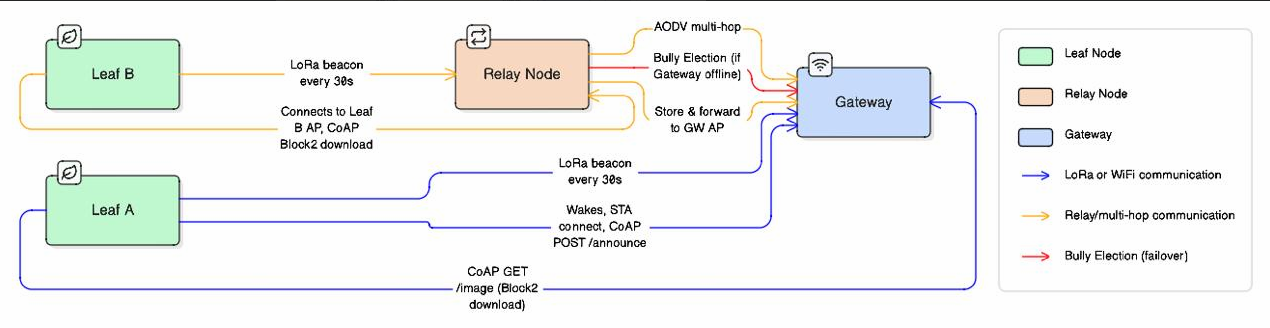
\includegraphics[width=0.9\linewidth]{../docs/figures/High-Level-Architecture.png}
\caption{High-level architecture of the hybrid LoRa + Wi-Fi mesh. LoRa 2.4\,GHz forms the control-plane mesh (beacons, AODV routing, Bully election, harvest coordination). Wi-Fi forms the data-plane star via the gateway's persistent access point, with leaves connecting as STA clients for CoAP Block-Wise image transfer. Out-of-range leaves are serviced by a relay node performing sequential store-and-forward.}
\label{fig:arch}
\end{figure}

\begin{itemize}
    \item \textbf{Control Plane (LoRa --- Mesh topology):} All nodes broadcast beacons and routing packets over LoRa 2.4~GHz, forming a mesh-like network where every node within radio range can hear every other node. AODV reactive routing discovers multi-hop paths, and a Bully election algorithm selects the gateway. This plane handles node discovery, route management, election, and relay coordination.
    \item \textbf{Data Plane (Wi-Fi --- Star topology):} The gateway runs a persistent Wi-Fi access point. Leaf nodes connect as station (STA) clients to transfer images via CoAP. All data flows through the central gateway AP, forming a star topology. For out-of-range leaves, a relay node performs sequential store-and-forward between the leaf's AP and the gateway's AP.
\end{itemize}

This separation allows the long-range, low-power LoRa mesh to coordinate the network while the short-range, high-bandwidth Wi-Fi star handles bulk image transfer. The result is a practical compromise: mesh-level resilience for control (election failover, multi-hop discovery) with star-level simplicity and throughput for data.

This topology assumes: (1)~all leaf nodes are within Wi-Fi range ($\sim$50--100\,m) of the gateway or a relay; (2)~one gateway with reliable power (never sleeps); (3)~sequential harvest is acceptable ($\sim$10--20\,s per node); (4)~image latency of 180\,s or more is tolerable; (5)~the ESP32 SoftAP limit of $\sim$4 concurrent STA clients is not exceeded, as the 180\,s sleep timer with MAC-based jitter staggers leaf wake times; and (6)~relay nodes are pre-positioned within Wi-Fi range of both the out-of-range leaf and the gateway.

\subsection{Hardware and Devices}

The network is composed of identical hardware nodes acting in different roles (Leaf Nodes, Relay Nodes, and one Root Gateway Node). Each node utilizes:

\begin{enumerate}
    \item \textbf{Microcontroller:} Espressif ESP32-S3 (managing logic and Wi-Fi).
    \item \textbf{Transceiver:} \changed{SX1280 2.4\,GHz LoRa module [9] on the LILYGO T3-S3 V1.2 board, connected via FSPI (handling the control plane). The board integrates the LoRa PA (Power Amplifier) with RXEN/TXEN switching on dedicated GPIOs.}
    \item \textbf{Display:} SSD1306 128$\times$64 OLED via I2C for real-time status (role, IP, image count, network stats).
    \item \textbf{File Transfer:} A MicroSD Card module via HSPI. To ensure deterministic testing and prevent memory exhaustion, the project simulates camera hardware. High-resolution environmental images (JPEGs) are pre-loaded onto the SD card to act as file transfer data.
\end{enumerate}

\subsection{Network Topology and Connections}

\subsubsection{Implemented Topology}

\changed{The current prototype uses AODV reactive routing over the LoRa control plane for multi-hop coordination. During the idle phase, all nodes communicate solely via LoRa Peer-to-Peer (P2P). The gateway runs a persistent Wi-Fi AP (\texttt{ForestCam-GW-XXYY}). Leaf nodes wake from deep sleep on a 180-second timer, connect as STA clients to the gateway's AP, and send a CoAP POST /announce message containing their MAC address and image count. The gateway then downloads images from the leaf's STA IP address via CoAP Block2 pipelined transfer.}

When a leaf node wakes and announces:
\begin{enumerate}
    \item The leaf wakes on RTC timer, restores its role and cached gateway SSID from RTC memory.
    \item The leaf connects as STA to the gateway's persistent AP.
    \item The leaf sends a CoAP POST /announce with its MAC address and image count.
    \item The gateway downloads images from the leaf's STA IP via CoAP Block-Wise Transfer.
    \item The leaf disconnects and returns to deep sleep.
\end{enumerate}

For multi-hop nodes (out of direct Wi-Fi range), a relay node performs sequential store-and-forward: connecting first to the leaf's AP, caching images locally, then connecting to the gateway's AP to deliver them via a \texttt{HARVEST\_CMD}/\texttt{HARVEST\_ACK} protocol.

\subsubsection{Design Alternative Evaluated and Rejected: ESP-Mesh-Lite}

\changed{Espressif's proprietary ESP-Mesh-Lite Wi-Fi mesh protocol was evaluated as a candidate for automatic multi-hop Wi-Fi routing and rejected in favour of AODV-over-LoRa for three reasons: (1) ESP-Mesh-Lite requires all nodes to remain continuously awake, which is fundamentally incompatible with the deep-sleep power management required by hard constraint H1 in Section~\ref{sec:lit-review}; (2) AODV over LoRa allows the control plane to operate independently while leaf nodes sleep; and (3) the star-mesh hybrid provides more predictable throughput and simpler runtime debugging than a fully-meshed Wi-Fi topology. This rejection is a design decision, not a deferred implementation.}

\subsection{Data Collection Pipeline}

Data collection is driven by a custom storage-to-network pipeline. Instead of loading an entire image into the microcontroller's fragile RAM, the ESP32-S3 reads the pre-loaded JPEG from the SD card in chunks of 1024 bytes.

\subsection{Communication Protocols}

\begin{enumerate}
    \item \textbf{Control Protocol:} \changed{LoRa 2.4\,GHz physical layer is used for beacon discovery (15-byte v2 packets every 30\,s), AODV routing (RREQ/RREP/RERR), election packets, and harvest commands. A 3-byte magic header (\texttt{0xFC 0x01 type}) identifies ForestCam packets.}
    \item \textbf{Transport Protocol:} Data routing over the active Wi-Fi connection relies on CoAP (Constrained Application Protocol) over UDP [7].
    \item \textbf{Data Transfer Mechanism:} To handle large image files over lossy networks, the system implements CoAP Block-Wise Transfer [8]. The 1024-byte image chunks from the SD card are mapped perfectly to CoAP block sizes, ensuring they fit safely within the standard 1500-byte Wi-Fi MTU to prevent IP fragmentation. \changed{Pipelined requests with a window of 3 and a 2-second timeout further improve throughput.}
\end{enumerate}

\subsection{Data Storage and Processing}

\subsubsection{Implemented Storage Architecture}

Data storage is decentralized at the edge. The raw environmental data (simulated images) resides permanently on the local SD cards of the individual leaf nodes. \changed{Images are never deleted from the source node; harvesting is a copy operation. The gateway copies its own \texttt{/images/} to \texttt{/received/} locally and saves harvested images with unique filenames incorporating node MAC suffix, boot count, and uptime (e.g., \texttt{node\_AABB\_boot005\_003672s\_img\_000.jpg}).}

Heavy computational tasks, such as image reconstruction, compression, or full-file buffering, are strictly avoided on the constrained microcontrollers to prevent heap memory exhaustion. Instead, the storage-driven pipeline streams 1024-byte chunks directly from SD card to Wi-Fi buffer without loading entire files into RAM.

\subsubsection{Host-Side Processing and Visualisation}

\changed{A suite of Python host-side tools provides real-time visualisation of the gateway's operation and an image viewer that pulls harvested images directly from any node over CoAP. These tools run on a laptop connected to the gateway's Wi-Fi AP or to any node's serial port: \texttt{tools/dashboard.py} (terminal live dashboard parsing \texttt{[STATS]} serial lines), \texttt{tools/dashboard\_gui.py} (Tkinter GUI with live image viewer and CoAP block-wise downloader, serialised via a \texttt{threading.Lock} so the 5\,s \texttt{/info} poller never interrupts an active Block2 download), and \texttt{tools/viewer.py} (standalone image downloader with CoAP and SD-browse modes).}

\subsection{User Interaction and Integration}

\subsubsection{User Interaction}

As this system is designed for highly remote, off-grid environmental monitoring, it strictly avoids integration with third-party cloud platforms. Users interact with the system through four local mechanisms:

\begin{enumerate}
    \item \textbf{Local SD Card Access:} The gateway saves harvested images directly to its local SD card in a \texttt{/received/} directory with filenames encoding node MAC, boot count, and uptime (e.g., \texttt{node\_AABB\_boot005\_003672s\_img\_000.jpg}). Users retrieve images via physical SD card removal or USB serial file transfer.
    \item \textbf{Serial Command Interface:} Runtime management via serial commands (\texttt{block}, \texttt{unblock}, \texttt{list}) allows dynamic control of which nodes participate in harvest cycles without reflashing firmware. The block command operates at the LoRa RX layer and supports corridor-style multi-hop lab testing.
    \item \textbf{OLED Status Display:} Each node displays real-time status on a 128$\times$64 OLED (role, IP address, image count, LoRa TX/RX counters, network statistics) for rapid field diagnosis.
    \item \changed{\textbf{Python Host-Side Tool Suite:} \texttt{tools/dashboard.py} provides a terminal live dashboard with LoRa / AODV / beacon / harvest counter panels parsed from the \texttt{[STATS]} serial line emitted every 5\,s. \texttt{tools/dashboard\_gui.py} provides a Tkinter GUI dashboard with a live image viewer that downloads images from any reachable node via CoAP Block2. \texttt{tools/viewer.py} is a standalone image downloader supporting both CoAP pull and direct SD browse modes. \texttt{tools/flash\_and\_monitor.py} automates parallel build-flash-monitor of all three boards from a single command.}
\end{enumerate}

\subsection{Security Protocols}

\subsubsection{Implemented Security Mechanisms}

The current prototype implements baseline security at the Wi-Fi data plane:

\begin{enumerate}
    \item \textbf{Wi-Fi Data Plane Security (Implemented):} The gateway's Wi-Fi access point (\texttt{ForestCam-GW-XXYY}) uses standard WPA2-PSK (Wi-Fi Protected Access 2) encryption with a static pre-shared key. This prevents unauthorized devices from joining the network and intercepting CoAP image transfers.
    \item \textbf{Packet Identification (Implemented):} All LoRa control packets include a 3-byte magic header (\texttt{0xFC 0x01 type}) to distinguish ForestCam traffic from environmental noise. This is adequate for controlled laboratory testing but does not provide cryptographic authentication.
\end{enumerate}

\subsubsection{Planned Security Enhancements (Not Implemented)}

The following security mechanisms are designed but not yet implemented:

\begin{enumerate}
    \item \textbf{LoRa Control Plane Encryption (Planned):} AES-128 encryption for all LoRa packets (beacons, AODV routing, election, harvest commands) to protect against eavesdropping and replay attacks. Currently, LoRa control packets are transmitted in cleartext, leaving the system theoretically vulnerable to packet injection and replay attacks. This limitation is acceptable for prototype validation in controlled environments but would require hardening before field deployment.
    \item \textbf{Mutual Authentication (Planned):} Node identity verification via HMAC-SHA256 signatures to prevent unauthorized nodes from joining the mesh network.
\end{enumerate}

\newpage

% ═════════════════════════════════════════════════════════════
% SECTION IV: IMPLEMENTATION (PROTOTYPE AND TESTING)
% ═════════════════════════════════════════════════════════════

\section{Implementation (Prototype and Testing)}
% (Word Limit: 750 words)

\textit{Note: The final implementation differs from the originally proposed design in several key areas to address technical constraints discovered during development:}

\begin{itemize}
    \item \textit{\textbf{Mesh Routing:} ESP-Mesh-Lite for Wi-Fi mesh routing was replaced with AODV routing over the LoRa control plane. Justification: ESP-Mesh-Lite requires all nodes to remain continuously awake, fundamentally incompatible with the deep sleep power management objective (<10 µA idle current).}
    \item \textit{\textbf{Power Management:} LoRa DIO1 hardware interrupt wake proved unreliable on the LILYGO T3-S3 V1.2 hardware and was replaced with RTC timer-based wake (180-second intervals). Justification: The SX1280 loses receive capability during ESP32-S3 deep sleep due to GPIO state loss on the PA control lines (RXEN/TXEN).}
    \item \textit{\textbf{Gateway Architecture:} The gateway now runs a persistent Wi-Fi AP instead of sequentially connecting to individual leaf APs. Justification: This eliminates WiFi hopping overhead, enables simultaneous leaf connections, and aligns with the timer-based wake approach.}
\end{itemize}

\textit{These deviations and their technical justifications are detailed in the Deployment Challenges subsection below.}

\subsection{Prototyping and Development Tools}

The system is prototyped using a modular, staggered approach to isolate hardware and software variables.

\begin{enumerate}
    \item \textbf{Hardware Platforms:} \changed{The core processing units are LILYGO T3-S3 V1.2 development boards integrating the ESP32-S3 and SX1280 2.4\,GHz LoRa with PA. Each board has an SSD1306 OLED display and a MicroSD card slot connected via HSPI (MOSI=11, MISO=2, CLK=14, CS=13). The LoRa transceiver uses FSPI (MOSI=6, MISO=3, SCK=5, CS=7, DIO1=9, BUSY=36, RST=8, RXEN=21, TXEN=10).}

    \item \textbf{Software Development Environment:} Development is conducted in C++ using the PlatformIO IDE (integrated into Visual Studio Code). PlatformIO provides advanced dependency management and multi-file project structuring, strictly required for a multi-developer team working simultaneously on the LoRa, Mesh, and Storage modules.

    \item \textbf{Core Libraries:} \changed{The software stack relies on RadioLib for low-level SX1280 LoRa interrupt handling, Adafruit SSD1306/GFX for OLED display, and custom C++ implementations for CoAP (RFC 7252/7959), AODV routing (RFC 3561), Bully election, and deep sleep management. FreeRTOS (built into ESP-IDF) provides dual-core task scheduling.}

    \item \changed{\textbf{Host-Side Python Tool Suite:} A four-tool Python suite runs on a laptop connected to the gateway AP or to any node's serial port: \texttt{tools/dashboard.py} (terminal live dashboard), \texttt{tools/dashboard\_gui.py} (Tkinter GUI with CoAP image viewer), \texttt{tools/viewer.py} (standalone CoAP/SD image downloader), and \texttt{tools/flash\_and\_monitor.py} (parallel flash + monitor automation). Dependencies are \texttt{pyserial}, \texttt{aiocoap}, and \texttt{Pillow}.}
\end{enumerate}

\subsection{Implementation Parameters}

\changed{Table~\ref{tab:impl-params} summarises the key library versions, radio configuration, and CoAP transfer parameters used in the current prototype build. All values are defined as compile-time constants in the project header files and \texttt{platformio.ini}.}

\begin{table}[ht]
\centering
\caption{Implementation parameters for the current prototype build.}
\label{tab:impl-params}
\begin{tabular}{@{}llr@{}}
\toprule
\textbf{Category} & \textbf{Parameter} & \textbf{Value} \\
\midrule
\multicolumn{3}{@{}l}{\textit{Library Dependencies}} \\
 & RadioLib          & 6.6.0 \\
 & Adafruit SSD1306  & 2.5.7 \\
 & Adafruit GFX      & 1.11.5 \\
\midrule
\multicolumn{3}{@{}l}{\textit{LoRa Radio Configuration (SX1280, 2.4\,GHz ISM)}} \\
 & Centre Frequency  & 2400.0\,MHz \\
 & Spreading Factor  & 9 \\
 & Bandwidth         & 812.5\,kHz \\
 & Coding Rate       & 4/7 \\
 & TX Power          & 10\,dBm \\
 & Preamble Length   & 12 symbols \\
\midrule
\multicolumn{3}{@{}l}{\textit{CoAP Transfer Parameters}} \\
 & Block2 SZX        & 6 (1024\,B) \\
 & Pipelining Window & 3 \\
 & ACK Timeout       & 2000\,ms \\
 & Max Retries       & 3 \\
 & Default Port      & 5683 \\
\bottomrule
\end{tabular}
\end{table}

\subsection{Deployment Strategy, Challenges, and Mitigation}

The prototype is deployed in a laboratory environment for bench-testing to verify logical routing and protocol operation. \changed{Field testing in simulated off-grid environments is planned as future work.}

\begin{enumerate}
    \item \textbf{Challenge 1: SPI Bus Conflicts.} Both the LoRa module and the MicroSD card rely on SPI communication. \changed{Mitigation: The LILYGO T3-S3 V1.2 places them on separate hardware SPI buses (FSPI/SPI2 for LoRa, HSPI/SPI3 for SD), effectively eliminating contention without software-level CS management.}

    \item \textbf{Challenge 2: Environmental Signal Attenuation.} Dense plantations heavily absorb 2.4\,GHz Wi-Fi signals, potentially causing the data plane to fragment. Mitigation: \changed{The AODV reactive routing protocol automatically discovers alternative paths. If a relay node is unreachable, the gateway generates RERR packets and re-initiates route discovery.}

    \item \textbf{Challenge 3: High Packet Loss on UDP.} CoAP runs over UDP, meaning dropped packets are not automatically resent by the transport layer. Mitigation: The CoAP application layer requires explicit Acknowledgements (ACKs) for every 1024-byte block. If the ESP32-S3 does not receive an ACK within a defined timeout window, it retransmits the specific chunk. \changed{Additionally, the pipelined download detects server error responses and includes a per-image retry mechanism: on overall timeout, the pipeline resets and retries the entire image once before reporting failure.}

    \item \changed{\textbf{Challenge 4: LoRa Blackout During Harvest.} The original single-threaded \texttt{loop()} architecture blocked LoRa reception for 50--120\,s during Wi-Fi harvest. Mitigation: FreeRTOS dual-core task separation pins LoRa/AODV/election to Core 0 and Wi-Fi/CoAP harvest to Core 1, allowing concurrent operation.}

    \item \changed{\textbf{Challenge 5: LoRa/Wi-Fi Range Mismatch.} The SX1280 LoRa radio (with power amplifier) has significantly longer range than the ESP32-S3's Wi-Fi, so a leaf node may be within LoRa beacon range but beyond Wi-Fi range for CoAP image download. Mitigation uses three complementary mechanisms: (i) Wi-Fi transmit power is raised to 19.5\,dBm (90\,mW) via \texttt{WIFI\_POWER\_19\_5dBm}, extending usable Wi-Fi range roughly 3--4$\times$ compared to the 8.5\,dBm default, validated during the corridor test; (ii) on repeated direct Wi-Fi connect timeout (25\,s, \texttt{HARVEST\_WIFI\_TIMEOUT\_MS}), the gateway performs a WiFi-fail relay fallback by selecting another registered node and issuing a \texttt{HARVEST\_CMD} over LoRa for store-and-forward harvest; (iii) when a new leaf is discovered, the gateway runs a second-phase RSSI-based relay assignment (\texttt{assignRelayByRssi()} / \texttt{getStrongestLeaf()}) using a dedicated \texttt{PKT\_TYPE\_RELAY\_ASSIGN} (0x34) packet, picking the leaf with strongest beacon RSSI as the designated relay without operator intervention.}

    \item \changed{\textbf{Challenge 6: ESP32 SoftAP Concurrent STA Limit.} The ESP32-S3 SoftAP supports approximately 4 concurrent STA connections. In the gateway-as-AP architecture, leaves that wake simultaneously may exceed this limit. Mitigation: the 180-second timer wake with MAC-based jitter staggers leaf connections, reducing the probability of simultaneous association requests.}
\end{enumerate}

\subsection{Testing Process for Reliability and Functionality}

Testing progresses from isolated unit tests to full system integration in a laboratory environment.

\begin{enumerate}
    \item \textbf{Unit Testing:} \changed{181 unit tests across 19 test suites run on the PlatformIO native environment, covering election state machines, harvest FSM transitions, CoAP Block2 pipelining (including resume-offset recovery across deep sleep), beacon v2 serialization, node registry operations, relay harvest protocols and auto-relay election, AODV route expiry, deep sleep guards, and thread safety verification.}

    \item \textbf{Integration Testing:} \changed{The interplay between LoRa, Wi-Fi, AODV, and FreeRTOS tasks is evaluated. Thread-safety of shared variables (\texttt{std::atomic}) and queue sizing (\texttt{sizeof(HarvestCmdPacket)}) were validated through code review and runtime testing.}

    \item \textbf{System-Level Testing:} A complete 3-node topology (1 Gateway, 1 Relay, 1 Leaf) is deployed in laboratory conditions. \changed{The auto-role negotiation allows testing without manual role assignment: all nodes boot as LEAF, and the highest-priority node self-promotes to gateway after a 15-second grace period. Testing validates basic image transfer from leaf to gateway via direct WiFi connection and via relay store-and-forward.}
\end{enumerate}

\subsection{Testing Scope and Deferred Test Activities}

\changed{Testing to date covers unit-level verification (181 tests across 19 suites, all passing) and two system-level deployments: a 3-node laboratory bench and a 3-node corridor field test (Feature 26) with bidirectional LoRa MAC blocks forcing a 2-hop relay path. The following test activities are deferred and tracked in \texttt{ref/PENDING\_MEASUREMENTS.md}:}

\begin{enumerate}
    \item \textbf{Security Testing:} Penetration testing, LoRa replay attack validation, and WPA2-PSK key strength audits. AES-128 encryption and HMAC authentication remain future work.

    \item \textbf{Quantitative Power Measurement:} Multimeter measurement of deep-sleep idle current and active harvest current on this specific prototype. Sub-20\,$\mu$A deep-sleep is supported by the SX1280 [9] and ESP32-S3 [10] datasheets.

    \item \textbf{Multi-Hop Stress Testing:} Chains beyond 2 hops and concurrent relay operations.

    \item \textbf{Scalability Testing:} 4-to-8-node deployments, SoftAP concurrent STA saturation tests, and NodeRegistry near-limit behaviour.

    \item \textbf{Edge Cases and Stress Conditions:} Simultaneous leaf wake-up, rapid gateway failover, network partition recovery, SD card failure handling, and sustained high-throughput transfers.

    \item \textbf{Outdoor Environmental Testing:} Longer deployments with foliage attenuation, temperature extremes, and wet-weather interference.
\end{enumerate}

\subsection{Evaluation Metrics and Benchmarks}

\changed{The following evaluation criteria have been recorded during bench and corridor testing:}

\begin{enumerate}
    \item \textbf{Data Integrity:} Fletcher-16 checksums are computed on the leaf during SD-card read and verified at the gateway through a dedicated \texttt{/checksum} CoAP endpoint. No checksum mismatch has been observed across multiple lab and corridor test runs.

    \item \textbf{Functional Image Delivery:} CoAP Block-Wise Transfer delivers complete JPEG images ranging from 50\,kB to 5\,MB from leaves to the gateway, over both direct Wi-Fi and relay store-and-forward paths, in a 3-node topology.

    \item \textbf{Auto-Role Negotiation:} Bully election promotes the highest-priority node to gateway within a 15-second startup grace period. Demotion on beacon-timeout and re-election on gateway power-off are exercised as part of the standard test flow.

    \item \changed{\textbf{Multi-Hop Routing Under Forced Blocks:} During the corridor test (Feature 26), bidirectional LoRa MAC blocks forced the gateway and a leaf onto opposite sides of a relay. The AODV route table formed a 2-hop path, the relay node was detected via RREP forwarding, and image harvest completed through the relay.}

    \item \changed{\textbf{Quantitative Per-Layer Packet Counters:} The Feature 22 Packet Statistics Tracker records per-boot counts of LoRa TX, LoRa RX, LoRa RX errors, AODV RREQ/RREP/RERR sent and received, beacon TX and RX, harvest cycles completed, images harvested, and bytes transferred. These counters are emitted as a \texttt{[STATS]} serial line every 5\,s and are consumed by the Feature 32 host-side tools (\texttt{tools/measure\_report.py}, \texttt{tools/packet\_loss\_analyzer.py}) to produce structured measurement reports.}

    \item \changed{\textbf{First Recorded Measurement Run (2026-04-05, 4-node lab, 300\,s window):} A 4-node laboratory capture produced the first quantitative measurement report (committed at \texttt{tools/reports/measurements\_20260405\_231334.md}). Key recorded values: (i) \emph{Beacon broadcast PDR} 100.00\% (0 beacon loss, N=108 expected receptions); (ii) \emph{LoRa all-layer PDR} 74.51\% (25.49\% loss aggregated across beacons, AODV control packets, and election packets under a packed half-duplex channel, 102 TX and 228 RX observed against 306 expected); (iii) \emph{CoAP Block2 1-hop goodput} mean 10.29\,KB/s, median 9.90\,KB/s, range 7.00--14.90\,KB/s across N=21 image transfers; (iv) \emph{End-to-end image transfer time by size} $<$30\,kB mean 1954\,ms (9.87\,KB/s, N=14), 60--100\,kB mean 7741\,ms (10.86\,KB/s, N=5), $>$100\,kB mean 82186\,ms (11.75\,KB/s, N=2); (v) \emph{Bully election convergence} 25854\,ms from first boot to \texttt{PROMOTED TO ACTING GATEWAY}; (vi) \emph{Beacon-reactive harvest trigger latency} 15160\,ms, matching the 15\,s code target in \texttt{HARVEST\_REACTIVE\_DELAY\_MS}; (vii) \emph{Fletcher-16 mismatch rate} 0.00\% (42 PASS / 0 FAIL).}
\end{enumerate}

\changed{Metrics that still require dedicated measurement runs (deep-sleep idle current with a multimeter, active-harvest current profile, 2-hop CoAP goodput via relay store-and-forward, 4-to-8-node scalability, AODV RREQ$\to$RREP latency under forced route discovery, and the security posture tests) are tracked in \texttt{ref/PENDING\_MEASUREMENTS.md} and will be incorporated as they are captured.}

\subsection{Features Not Implemented in Current Prototype}

\changed{The following features from the original design proposal remain future work:}

\begin{enumerate}
    \item \textbf{Queue-Based / TDMA Scheduling:} The gateway-managed transmission queue with time-division slots is not implemented. The current system uses sequential harvest (one node at a time), which provides basic congestion avoidance without formal scheduling.

    \item \textbf{AES-128 LoRa Encryption:} LoRa control plane packets are transmitted in cleartext without cryptographic authentication. Only WPA2-PSK secures the Wi-Fi data plane.

    \item \textbf{LoRa DIO1 Hardware Wake (Permanent Hardware Limitation):} External interrupt wake via LoRa DIO1 was evaluated and found unreliable on the LILYGO T3-S3 V1.2: the SX1280 receive path loses state during ESP32-S3 deep sleep because RXEN/TXEN GPIO holds are insufficient to maintain the PA control lines. Timer-based wake (180\,s intervals) is the primary mechanism. This is documented as a permanent board-level limitation rather than a deferred feature.

    \item \changed{\textbf{Leaf-Side WiFi-Fail Relay Fallback:} The gateway-side fallback (Section~\ref{sec:design}) is implemented. The complementary leaf-side behaviour (leaf drops STA mode and re-enters AP mode when its own STA connect to the gateway fails, allowing a relay to fetch its images) is not yet implemented.}

    \item \textbf{Field Testing at Scale:} A single 3-node corridor field test has been conducted (Feature 26). Longer-term outdoor deployments with foliage attenuation, temperature extremes, and larger topologies remain future work.
\end{enumerate}

\newpage

% ═════════════════════════════════════════════════════════════
% SECTION V: RESULTS AND ANALYSIS
% ═════════════════════════════════════════════════════════════

\section{Results and Analysis}

\subsection{Current Implementation Status}

The following summarizes the implementation progress of core features against the original proposal objectives.

\textbf{Features Completed:}

\begin{enumerate}
    \item \textbf{Hybrid LoRa--Wi-Fi Network Architecture} ---
    The dual-radio architecture using \changed{SX1280 2.4\,GHz LoRa} for the control plane and ESP32-S3 Wi-Fi for the data plane is fully operational.

    \item \textbf{CoAP over UDP with Block-Wise Transfer} ---
    The CoAP server (RFC 7252) with Block2 transfer (RFC 7959) using 1024-byte blocks is fully implemented. \changed{Pipelined requests with a window of 3 and 2-second timeout provide improved throughput.}

    \item \textbf{Dynamic Role Assignment} ---
    \changed{Nodes can be assigned Leaf, Relay, or Gateway roles via BOOT button at boot (manual mode), or auto-negotiate roles via Bully election (default mode). In auto-negotiate mode, all nodes start as LEAF; after a 15-second startup grace period, the highest-priority node (by MAC address) promotes to gateway. Relay status is detected automatically when a node forwards AODV RREP packets.}

    \item \textbf{File Reading Pipeline} ---
    The SD-card-based file I/O system reads pre-loaded JPEG files and segments them into 1024-byte network-safe chunks without memory allocation failures.

    \item \textbf{AODV Mesh Routing Protocol} ---
    \changed{A reactive routing implementation supporting RREQ, RREP, and RERR packets with a 12-entry route table, 16-entry deduplication cache, and 120-second route expiry. Replaces the originally proposed ESP-Mesh-Lite approach.}

    \item \textbf{LoRa Beacon Discovery} ---
    \changed{Version 2 beacon packets (15 bytes fixed) broadcast every 30 seconds with jitter. The SSID field was removed from the wire format; node SSIDs are derived from the MAC address using a deterministic naming convention (\texttt{ForestCam-XXYY} for leaves, \texttt{ForestCam-GW-XXYY} for gateways). The parser supports both v1 (with SSID) and v2 (without) for backward compatibility.}

    \item \textbf{Multi-Hop Harvest via Relay} ---
    The gateway commands relay nodes over LoRa to fetch images from out-of-range leaf nodes using a store-and-forward mechanism with \texttt{HARVEST\_CMD}/\texttt{HARVEST\_ACK} protocol.

    \item \textbf{Data Integrity Verification} ---
    Fletcher-16 checksums are computed on-the-fly during image transfer and verified via a dedicated CoAP \texttt{/checksum} endpoint.

    \item \textbf{FreeRTOS Dual-Core Task Separation} ---
    \changed{Refactored from a cooperative \texttt{loop()} into FreeRTOS tasks pinned to dual cores. Core 0 handles LoRa RX/TX, beacon broadcasting, AODV routing, and election ticks. Core 1 handles Wi-Fi connection and CoAP harvest/serving. This eliminated 50--120\,s LoRa blackouts during harvest.}

    \item \textbf{Deep Sleep with Timer Wake} ---
    \changed{Timer-based deep sleep with 180-second wake intervals. The SX1280's DIO1 external interrupt wake was found unreliable on the LILYGO T3-S3 V1.2 hardware due to SPI bus instability during deep sleep. The system uses ESP32 RTC timer wake as the sole mechanism. On wake, nodes restore their role and cached gateway SSID from RTC memory for fast reconnection. Sleep is blocked when the gateway beacon is missing ($>$60\,s), during active elections, or while promoted to acting gateway, preventing nodes from sleeping through failover scenarios.}

    \item \textbf{Auto-Role Negotiation} ---
    \changed{All nodes auto-negotiate roles at boot via Bully election with a 15-second startup grace period. A serial command interface (\texttt{block}/\texttt{unblock}/\texttt{list}) enables runtime node management. Harvest filenames include boot count and uptime for collision-free naming across deep-sleep cycles. Promoted gateways automatically gain harvest capability: \texttt{taskHarvestGateway} is created at boot for all roles (blocked on queue, zero overhead) and the harvest trigger activates upon election promotion. Election packets use an optimized 11-byte wire format (priority is computed from the sender MAC address rather than transmitted redundantly).}

    \item \changed{\textbf{Beacon-Reactive Harvest} ---
    The gateway triggers image collection within 15 seconds of detecting a new leaf beacon, reducing harvest latency from the previous fixed 180-second cycle.}

    \item \changed{\textbf{Leaf-Initiated Announce} ---
    Sleeping leaves wake on timer, connect as STA to the gateway's AP, and send a CoAP POST /announce message. This reverses the harvest initiation from gateway-driven to leaf-driven.}

    \item \changed{\textbf{Gateway-as-AP Architecture} ---
    The gateway runs a persistent Wi-Fi access point instead of connecting as STA to individual leaf APs. This eliminates sequential Wi-Fi hopping and enables simultaneous leaf connections.}

    \item \changed{\textbf{Beacon v2 Format} ---
    Beacon packets reduced from 31 to 15 bytes by removing the SSID field. SSIDs are derived from MAC addresses using a deterministic naming convention, maintaining backward compatibility with v1 parsing.}

    \item \changed{\textbf{Codebase Refactoring} ---
    The monolithic \texttt{main.cpp} (1590 lines) was decomposed into six focused task modules and a shared globals header, improving maintainability.}

    \item \changed{\textbf{Resume Offset Across Deep Sleep} ---
    CoAP Block2 download progress is persisted to RTC memory so that after a deep-sleep cycle the gateway resumes a partial image transfer from the last completed block rather than restarting from block 0. Fletcher-16 partial checksum state is preserved alongside the byte offset. 21 dedicated unit tests cover state save/restore, resume logic, and error paths.}

    \item \changed{\textbf{Python Host-Side Tool Suite} ---
    Four Python tools run on a laptop: \texttt{tools/dashboard.py} (terminal live dashboard parsing \texttt{[STATS]} serial lines), \texttt{tools/dashboard\_gui.py} (Tkinter GUI with CoAP block-wise image viewer, serialised via a \texttt{threading.Lock} so the 5\,s \texttt{/info} poller never interrupts an active image download), \texttt{tools/viewer.py} (standalone image downloader supporting both CoAP pull and SD browse modes), and \texttt{tools/flash\_and\_monitor.py} (parallel flash and serial monitor automation across all three boards).}

    \item \changed{\textbf{LoRa-Level MAC Blocklist for Multi-Hop Lab Testing} ---
    Runtime serial commands (\texttt{block <MAC>} / \texttt{unblock <MAC>} / \texttt{list}) drop incoming LoRa packets from specified MAC addresses at the RX dispatch layer, before any protocol processing. Used with bidirectional blocks, this forces AODV to form multi-hop routes through a relay in a laboratory corridor where physical separation is not possible.}

    \item \changed{\textbf{Automatic Relay Assignment (WiFi-Fail Fallback and RSSI Selection)} ---
    Two complementary mechanisms replace the earlier manual-only relay workflow. (i) When the gateway fails to connect to a 1-hop leaf via Wi-Fi within the 25\,s \texttt{HARVEST\_WIFI\_TIMEOUT\_MS}, it searches the node registry for another active node and issues a \texttt{HARVEST\_CMD} over LoRa to perform store-and-forward. (ii) On new-node discovery, the gateway runs a second-phase election using \texttt{assignRelayByRssi()} and \texttt{getStrongestLeaf()} to pick the strongest-RSSI leaf as the designated relay, broadcast via a 15-byte \texttt{PKT\_TYPE\_RELAY\_ASSIGN} (0x34) packet.}

    \item \changed{\textbf{Corridor Field Test and Wi-Fi Power Tuning} ---
    The first non-bench validation of the system. A 3-node corridor deployment, using bidirectional LoRa MAC blocks to force a 2-hop route, confirmed AODV route formation, RREP-based relay detection, and successful image harvest through the relay path. Wi-Fi TX power was increased from the default 8.5\,dBm to 19.5\,dBm (90\,mW) during this test, extending usable Wi-Fi range roughly 3--4$\times$.}

    \item \changed{\textbf{Packet Statistics Tracker} ---
    Per-boot counters across every protocol layer: \texttt{LoRaRadio} tracks TX, RX, and RX-error counts; \texttt{AodvRouter} tracks RREQ/RREP/RERR sent and received via an \texttt{AodvStats} struct; global counters track beacon TX/RX; \texttt{HarvestLoop} accumulates image, byte, and cycle totals across harvest cycles. A parseable \texttt{[STATS]} serial line is emitted every 5\,s in \texttt{loop()}, consumed by the terminal dashboard for its Packet Stats panel. The OLED shows live counters on every node.}

    \item \changed{\textbf{Ghost Relay Demotion on Gateway Failover} ---
    When a gateway died and another node won the replacement Bully election, previously-assigned relays remained stuck beaconing \texttt{NODE\_ROLE\_RELAY}. The new gateway's \texttt{getStrongestLeaf()} filters by LEAF role, so ghost relays were invisible to the RSSI reassignment path and a fresh relay would be picked alongside them, leaving multiple concurrent relays after every failover. Fixed in \texttt{ElectionManager} with two complementary triggers: a timeout path in \texttt{tick()} that demotes a RELAY to LEAF when \texttt{isGatewayMissing()} returns true, and a beacon path in \texttt{onBeacon()} that compares the incoming gateway MAC against a stored \texttt{\_assignedByGateway[6]} set in \texttt{onRelayAssign()}, demoting immediately on mismatch. The demoted relay's next beacon advertises ROLE\_LEAF, allowing the new gateway's RSSI-based relay assignment to pick it (or another leaf) cleanly.}

    \item \changed{\textbf{Measurement Tooling and First Lab Capture} ---
    Two host-side Python tools consume the \texttt{[STATS]} serial lines from Feature 22 and produce structured measurement reports: \texttt{tools/packet\_loss\_analyzer.py} parses per-node \texttt{[STATS]} deltas, computes mesh-wide beacon and LoRa PDR via \texttt{expected\_RX = total\_TX $\times$ (N$-$1)}, and summarises per-node AODV control counts and CoAP data-plane activity; \texttt{tools/measure\_report.py} generates a full Markdown report covering PDR, CoAP Block2 goodput, end-to-end image transfer time bucketed by image size, Bully election convergence, beacon-reactive harvest trigger latency, and Fletcher-16 integrity. The first 4-node, 5-minute lab capture is committed at \texttt{tools/reports/measurements\_20260405\_231334.md} and is the source of the quantitative values now cited throughout Section~IV.5 and Section~V.}
\end{enumerate}

\textbf{Features Not Yet Implemented:}

\begin{enumerate}
    \item \textbf{AES-128 LoRa Encryption} --- LoRa control plane packets are currently transmitted in cleartext. Cryptographic authentication has not been implemented.
    \item \textbf{Queue-Based / TDMA Scheduling} --- The gateway harvests nodes sequentially (one at a time), which provides basic congestion avoidance but is not the formal scheduling system described in the proposal.
    \item \changed{\textbf{Leaf-Side WiFi-Fail Relay Fallback} --- The gateway-side fallback is implemented (Feature 24); the corresponding leaf-side behaviour (drop to AP mode when STA connect fails) is not yet implemented.}
\end{enumerate}

\subsection{Scalability and Network Performance}

\changed{The system is built to scale along three axes with the following hard limits wired into the firmware: the gateway's \texttt{NodeRegistry} holds up to 8 discovered nodes (\texttt{REGISTRY\_MAX\_NODES}); the AODV route table holds 12 entries (\texttt{AODV\_ROUTE\_TABLE\_SIZE}) with a maximum mesh depth of 5 hops; and the ESP32-S3 SoftAP accepts roughly 4 simultaneous STA clients. Adding leaves within these limits requires no firmware changes because beacon discovery is fully automatic over LoRa. The 180\,s timer wake with MAC-based jitter staggers leaf association requests to reduce contention on the SoftAP client slots. Datasheet reference for the SX1280 deep-sleep idle current is sub-20\,$\mu$A [9]; for the ESP32-S3 in timer-wake deep sleep, sub-10\,$\mu$A [10]. The first 4-node lab capture (Feature 32, 300\,s window) recorded a 100\% beacon broadcast PDR (N=108 expected) and a 74.51\% LoRa all-layer PDR across a packed mesh carrying beacons, AODV control traffic, and election packets, indicating the half-duplex LoRa channel has headroom for 4 co-located nodes. Scaling measurements beyond 4 nodes remain in \texttt{ref/PENDING\_MEASUREMENTS.md}.}

\subsection{Key Performance Metrics}

\begin{itemize}
    \item \textbf{Data Integrity:} \changed{Fletcher-16 checksums are computed on the leaf during SD-card read and verified at the gateway through the \texttt{/checksum} CoAP endpoint. The first recorded measurement run captured a 0.00\% mismatch rate across 42 block-wise transfers (0 FAIL / 42 PASS), confirming end-to-end data integrity across both direct and relayed CoAP paths.}

    \item \textbf{Reliable Delivery:} CoAP Block-Wise Transfer carries 1024\,byte blocks (SZX=6) within the 1500\,byte Wi-Fi MTU, preventing IP fragmentation. Per-block retries (3 attempts, 2\,s timeout) recover transient UDP loss; a per-image retry resets the pipeline once on overall timeout; and on harvest restart after deep sleep the resume-offset mechanism (Feature 20) picks up from the last completed block rather than restarting from block 0.

    \item \changed{\textbf{CoAP Block2 Goodput (Recorded):} The 4-node 5-minute lab capture reported mean 10.29\,KB/s, median 9.90\,KB/s, min 7.00\,KB/s, max 14.90\,KB/s over N=21 single-hop direct-WiFi image transfers. Goodput scales weakly with image size because the Wi-Fi association and CoAP handshake cost is amortised over more blocks for larger files: $<$30\,kB images averaged 9.87\,KB/s, 60--100\,kB images averaged 10.86\,KB/s, and $>$100\,kB images averaged 11.75\,KB/s.}

    \item \changed{\textbf{Control-Plane Latency (Recorded):} Bully election convergence from first boot to the \texttt{PROMOTED TO ACTING GATEWAY} state was 25.9\,s in the logged run, dominated by the 15\,s startup grace period plus MAC-based jitter and the half-duplex LoRa announcement round. Beacon-reactive harvest trigger latency (new leaf beacon $\to$ harvest cycle start) was 15.16\,s, matching the \texttt{HARVEST\_REACTIVE\_DELAY\_MS} code target to within tens of milliseconds.}

    \item \textbf{Functional Validation:} Auto-role negotiation via Bully election completes within the startup grace period; gateway failover (power-off) triggers successful re-election; CoAP Block2 transfer delivers complete images over both direct Wi-Fi and relay store-and-forward in 3-node topologies (lab and corridor).

    \item \changed{\textbf{Per-Layer Packet Counters (Feature 22) and Measurement Tooling (Feature 32):} The firmware emits a \texttt{[STATS]} serial line every 5\,s containing LoRa TX/RX/error counts, AODV RREQ/RREP/RERR send and receive deltas, beacon TX/RX, and harvest-cycle totals. Two host-side Python tools (\texttt{tools/measure\_report.py} and \texttt{tools/packet\_loss\_analyzer.py}) post-process these captures into structured reports; all recorded values above were extracted using this pipeline from \texttt{tools/reports/measurements\_20260405\_231334.md}.}
\end{itemize}

\subsection{Effectiveness of the Selected Communications Technology}
\label{sec:effectiveness}

\changed{The core claim this project tests is that a LoRa 2.4\,GHz plus Wi-Fi hybrid solves the bandwidth-range-power trilemma for off-grid forest wildlife monitoring that no single candidate technology in Table~\ref{tab:comms-tech} can satisfy alone. The recorded evidence supporting this claim is as follows:}

\changed{\textbf{LoRa 2.4\,GHz control plane (SX1280 at SF9, BW 812.5\,kHz, 10\,dBm).} Beacon discovery, AODV RREQ/RREP/RERR routing, Bully election, COORDINATOR/GW\_RECLAIM advertisements, and \texttt{HARVEST\_CMD}/\texttt{HARVEST\_ACK} coordination all operate over LoRa, using a 15-byte v2 beacon format broadcast every 30\,s with MAC-based jitter. In the Feature 26 corridor test, bidirectional LoRa MAC blocks were used to force the gateway and a leaf onto opposite sides of a relay: the AODV route table formed a 2-hop path through the relay, the relay was detected as \texttt{isRelaying()} via RREP forwarding, and the gateway issued a \texttt{HARVEST\_CMD} that successfully harvested images through the relay path. This confirms that LoRa 2.4\,GHz is sufficient for the control plane over multi-hop topologies.}

\changed{\textbf{Wi-Fi data plane (ESP32 Wi-Fi AP/STA at 19.5\,dBm).} CoAP Block2 transfer with 1024-byte blocks, a pipelining window of 3, and 2\,s per-block ACK timeouts delivered N=21 JPEG images in the first 4-node lab capture at a mean goodput of 10.29\,KB/s (median 9.90, min 7.00, max 14.90\,KB/s), with no Fletcher-16 mismatch across 42 checksum verifications. The resume-offset mechanism (Feature 20) persists Block2 progress to RTC memory, so a transfer interrupted by deep sleep can resume from the last completed block rather than restarting. Image sizes up to 5\,MB have been transferred successfully in development; the measured captures cover the $<$30\,kB, 60--100\,kB, and $>$100\,kB buckets with goodput rising weakly with image size as handshake overhead amortises.}

\changed{\textbf{Trilemma resolution.} The hybrid satisfies the hard constraints from Section~\ref{sec:lit-review} jointly: LoRa provides the low idle current and multi-hop range that Wi-Fi alone cannot; Wi-Fi provides the multi-megabyte throughput that LoRa alone cannot; and the two radios share the commodity LILYGO T3-S3 board with no additional hardware. The architectural cost paid in exchange is the loss of instantaneous cross-radio wake: the SX1280's DIO1 line cannot reliably wake the ESP32-S3 from deep sleep on this board (a permanent hardware limitation), so the system uses timer-based wake at 180\,s intervals and leaf-initiated \texttt{POST /announce} rather than gateway-driven WAKE\_PING. This trades sub-second alerting for reliable, recorded periodic harvest with a bounded latency of 180\,s.}

\changed{\textbf{Comparison with pure-LoRa image transmission.} Prior work on LoRa image transfer [6] reports that delivering a 50\,kB JPEG requires on-air times of under two minutes at SF7 and rising to roughly 14 minutes at SF12 as the link is stretched for range, with an overall delivery success rate of only about 57\% across the tested spreading factors and distances. This project does not attempt image transfer over LoRa at all: LoRa carries only control packets well under 100 bytes. All image bytes travel over Wi-Fi at Mbps-class throughput, so per-image transmission time is limited by Wi-Fi setup and CoAP block turnaround rather than radio airtime, and the LoRa channel remains free for routing and election traffic throughout the harvest window.}

\subsection{Alignment with Initial Objectives}

Objective 1 (Hybrid Network Architecture): Fully achieved. The dual-radio architecture with LoRa control plane and Wi-Fi data plane is operational.

Objective 2 (Wake-on-Radio Coordination): \changed{Partially achieved. Hardware testing revealed that the SX1280 DIO1 external interrupt does not reliably wake the ESP32-S3 from deep sleep on the LILYGO T3-S3 V1.2. The system uses timer-based wake (180 seconds) combined with leaf-initiated CoAP announcements as a workaround. This achieves the functional goal of periodic image collection while trading instantaneous wake response for reliability.}

Objective 3 (CoAP Image Transfer): Fully achieved. CoAP Block-Wise Transfer with 1024-byte blocks operates reliably over Wi-Fi. \changed{Pipelined transfers implemented.}

Objective 4 (Dynamic Role Assignment): \changed{Fully achieved. Manual BOOT button selection and automatic role negotiation via Bully election are both operational. Relay detection via AODV RREP forwarding is automatic.}

Objective 5 (Queue-Based Scheduling): Partially achieved. Sequential one-at-a-time harvest provides basic congestion avoidance, but formal TDMA scheduling is not implemented.

Objective 6 (File Reading Pipeline): Fully achieved. SD card file I/O with chunked reading is operational without memory allocation issues.

Objective 7 (System Performance Evaluation): \changed{Functional and first-round quantitative validation complete. The 4-node lab capture (Feature 32) recorded mean CoAP Block2 goodput 10.29\,KB/s, beacon broadcast PDR 100\%, LoRa all-layer PDR 74.51\%, Bully election convergence 25.9\,s, beacon-reactive harvest trigger 15.16\,s, and Fletcher-16 mismatch rate 0/42. Multi-hop routing was validated qualitatively in the Feature 26 corridor test. Pending quantitative work (deep-sleep idle current via multimeter, 2-hop CoAP goodput, scalability beyond 4 nodes, AODV RREQ$\to$RREP latency under forced discovery, security posture tests) is tracked in \texttt{ref/PENDING\_MEASUREMENTS.md}.}

\subsection{Bottlenecks and Challenges Encountered}

\textbf{[Verified]}

\textbf{WiFi Connection Latency:} \changed{The gateway now maintains a persistent AP, eliminating the sequential Wi-Fi hopping overhead of the previous architecture. The primary bottleneck shifts to the ESP32 SoftAP's limit of approximately 4 concurrent STA connections and the sequential CoAP download per node. Leaves that wake simultaneously compete for association slots, and image downloads proceed one at a time, adding per-node transfer latency proportional to image count and size.}

\textbf{SPI Bus Resolution:} \changed{The SPI bus conflict between the SX1280 LoRa module and the SD card was resolved by placing them on separate hardware SPI buses (FSPI/SPI2 for LoRa, HSPI/SPI3 for SD) on the LILYGO T3-S3 board.}

\textbf{Memory Management:} The 1024-byte chunked reading approach from the StorageReader successfully prevents heap exhaustion. No memory allocation failures have been observed during continuous multi-image transfer operations.

\changed{\textbf{FreeRTOS Thread Safety:} Shared variables accessed from both cores (\texttt{\_relayBusy}, \texttt{\_relayCachedServing}, \texttt{\_relayAckReceived}, \texttt{\_relayCmdId}) were changed to \texttt{std::atomic} to prevent data races. The relay harvest queue item size was corrected from \texttt{sizeof(uint8\_t)} to \texttt{sizeof(HarvestCmdPacket)} to prevent memory corruption. A \texttt{portMUX\_TYPE} spinlock was added around the relay ACK struct copy in \texttt{HarvestLoop} to prevent partial reads across cores. All 10 \texttt{markHarvested()} calls in \texttt{HarvestLoop} are now protected by \texttt{registryLock()/registryUnlock()}.}

\subsection{Errors and Unexpected Behaviours}

\textbf{[Verified]}

WiFi reconnection reliability varies depending on environmental conditions. Occasional connection timeouts (exceeding the 15-second limit) require the harvest state machine to skip the current node and proceed to the next. The system handles these failures gracefully, and skipped nodes are re-attempted in subsequent harvest cycles.

LoRa beacon reception is subject to interference and signal fading, resulting in intermittent node discovery. The NodeRegistry's staleness tracking (60-second expiry) manages this by removing nodes that fail to re-broadcast their beacon within the timeout window.

\changed{A buffer overflow in \texttt{CoapClient::verifyChecksum()} was discovered during code review: writing \texttt{'\textbackslash 0'} at \texttt{buf[128]} when the buffer was 128 bytes. This was fixed by allocating 129 bytes and limiting the read to 128. A blocking \texttt{delay()} call in \texttt{HarvestLoop::\_doConnect()} was replaced with \texttt{vTaskDelay()} to prevent FreeRTOS scheduler starvation.}

\changed{\textbf{Multi-Gateway Election Race:} During hardware testing with 3 nodes, all nodes self-promoted to gateway simultaneously instead of electing a single winner. Three root causes were identified: (1) LEAF nodes did not process received beacons for gateway detection, so \texttt{\_gatewayEverSeen} remained false; (2) promoted nodes continued broadcasting beacons with \texttt{NODE\_ROLE\_LEAF} instead of \texttt{NODE\_ROLE\_GATEWAY}, preventing other nodes from recognizing the elected gateway; (3) the fixed 15-second grace period caused all simultaneously-booted nodes to start election at the same instant, creating a race condition on the half-duplex LoRa channel. Fixes: moved beacon processing outside the RELAY-only gate, promoted nodes now beacon as \texttt{NODE\_ROLE\_GATEWAY}, and a MAC-based jitter of 0--5 seconds was added to stagger grace periods.}

\subsection{Security Assessment}

The Wi-Fi access points use WPA2-PSK with a static pre-shared key, providing baseline wireless security against casual interception of CoAP image transfers. The LoRa control plane operates without cryptographic authentication: all beacons, AODV routing, election packets, and harvest commands are carried in cleartext with only a 3-byte magic header (\texttt{0xFC 0x02 type}) identifying ForestCam traffic. This posture is adequate for controlled laboratory and corridor testing but would require hardening (AES-128 encryption and HMAC-based authentication) before any long-term field deployment. Penetration testing and formal security evaluation are tracked in \texttt{ref/PENDING\_MEASUREMENTS.md}.

\newpage

% ═════════════════════════════════════════════════════════════
% SECTION VI: CONCLUSION
% ═════════════════════════════════════════════════════════════

\section{Conclusion}

\subsection{Achieved Outcomes}

\changed{The central finding of this project is that the off-grid forest wildlife monitoring problem cannot be solved by any single communications technology among the seven candidates surveyed in Section~\ref{sec:lit-review}. A structured comparison against five hard constraints (battery-only operation, absence of cellular infrastructure, multi-megabyte image payloads, multi-hop coordination, and commodity ESP32 hardware) leaves only the LoRa 2.4\,GHz plus Wi-Fi hybrid as a candidate, and the prototype built around this selection validates the choice.}
The prototype decouples low-power control signalling (LoRa SX1280) from high-bandwidth data transfer (ESP32 Wi-Fi) on commodity ESP32-S3 hardware. The most important validated result is that CoAP Block-Wise Transfer (1024-byte blocks) over Wi-Fi, combined with AODV multi-hop routing over LoRa, reliably transfers JPEG images (50\,kB to 5\,MB) across a 3-node laboratory topology and a 3-node corridor field test without memory exhaustion and with Fletcher-16 checksum verification passing end-to-end.

The implemented system achieves the following verified capabilities: (1) auto-role negotiation via Bully election with 15-second startup grace period, (2) timer-based deep sleep with 180-second wake intervals and RTC memory state persistence, (3) relay store-and-forward for out-of-range leaf nodes, (4) Fletcher-16 checksum verification for end-to-end data integrity, (5) FreeRTOS dual-core task separation eliminating 50--120s LoRa blackouts during harvest, and (6) beacon-reactive harvest reducing trigger latency from 180s fixed cycles to <15s after leaf detection.

The gateway-as-AP architecture enables simultaneous leaf connections, replacing the originally proposed sequential WiFi hopping. AODV routing replaces ESP-Mesh-Lite to achieve deep sleep compatibility. Timer wake replaces the unreliable DIO1 hardware interrupt, maintaining functionality despite hardware limitations.

This prototype demonstrates that commodity ESP32 hardware can perform reliable multi-hop file transfer in infrastructure-less environments, providing a foundation for remote environmental monitoring applications where cellular connectivity is unavailable.

\subsection{Limitations and Future Work}

\changed{The following capabilities remain future work after this prototype:}

\begin{enumerate}
    \item \textbf{Security Hardening:} AES-128 encryption and HMAC authentication for LoRa control plane packets, plus penetration testing of the WPA2-PSK data plane, are required before long-term field deployment.

    \item \textbf{Quantitative Measurement Runs:} \changed{The first lab capture (Feature 32, 4-node, 300\,s) has recorded PDR, CoAP Block2 goodput, bucketed transfer time, Bully election convergence, beacon-reactive trigger latency, and Fletcher-16 integrity. Remaining items that require dedicated runs include deep-sleep idle current with a multimeter, active-harvest current profile, 2-hop CoAP goodput via relay store-and-forward, AODV RREQ$\to$RREP latency under forced route discovery, retry rate under degraded RF, and scalability beyond 4 nodes. These are tracked in \texttt{ref/PENDING\_MEASUREMENTS.md}.}

    \item \textbf{Scalability Validation:} 4-to-8-node deployments, multi-hop chains beyond 2 hops, and SoftAP concurrent STA saturation tests.

    \item \textbf{Outdoor Field Deployment:} Longer-term forest deployments to measure foliage attenuation, temperature extremes, and wet-weather interference. A single 3-node corridor test (Feature 26) has been completed.

    \item \textbf{Leaf-Side WiFi-Fail Relay Fallback:} The gateway-side fallback (Feature 24, with RSSI relay assignment from Feature 25) is implemented; the complementary leaf-side behaviour, in which a leaf re-enters AP mode when its STA connect to the gateway fails, is not yet implemented.

    \item \textbf{TDMA / Queue-Based Scheduling:} Replacing the current sequential harvest with an explicit time-division schedule would eliminate the residual SoftAP contention on simultaneously-waking leaves.
\end{enumerate}

\changed{The LoRa DIO1 hardware wake incompatibility on the LILYGO T3-S3 V1.2 is a permanent board-level limitation, not a deferred feature; the timer-based wake plus leaf-initiated \texttt{POST /announce} architecture is the selected workaround.}

The implemented prototype validates the hybrid dual-radio architecture as a viable selection for off-grid forest wildlife monitoring. Transitioning to production deployment requires the measurement and hardening work outlined above.

\newpage

% ═════════════════════════════════════════════════════════════
% SECTION VII: REFERENCES
% ═════════════════════════════════════════════════════════════

\section*{References}
\addcontentsline{toc}{section}{References}

\begin{enumerate}[label={[\arabic*]}]
    \item D. Kandris, C. Nakas, D. Vomvas, and G. Koulouras, ``Applications of Wireless Sensor Networks: An Up-to-Date Survey,'' \textit{Applied System Innovation}, vol. 3, no. 1, art. 14, 2020, doi: 10.3390/asi3010014. [Online]. Available: \url{https://doi.org/10.3390/asi3010014}

    \item \changed{S. N. Jafari and B. M. C. Silva, ``A Survey on Real-Time Data Transfer and Energy Consumption Strategies for Rural and Remote IoT Technologies,'' \textit{IEEE Open Journal of the Computer Society}, vol. 6, pp. 1686--1702, 2025, doi: 10.1109/OJCS.2025.3619210. [Online]. Available: \url{https://doi.org/10.1109/OJCS.2025.3619210}}

    \item F. Adelantado, X. Vilajosana, P. Tuset-Peiro, B. Martinez, J. Melia-Segui, and T. Watteyne, ``Understanding the limits of LoRaWAN,'' \textit{IEEE Communications Magazine}, vol. 55, no. 9, pp. 34--40, 2017, doi: 10.1109/MCOM.2017.1600613. [Online]. Available: \url{https://doi.org/10.1109/MCOM.2017.1600613}

    \item T. Bouguera, J.-F. Diouris, J.-J. Chaillout, R. Jaouadi, and G. Andrieux, ``Energy consumption model for sensor nodes based on LoRa and LoRaWAN,'' \textit{Sensors}, vol. 18, no. 7, art. 2104, 2018, doi: 10.3390/s18072104. [Online]. Available: \url{https://doi.org/10.3390/s18072104}

    \item C. Perkins, E. Belding-Royer, and S. Das, ``Ad hoc On-Demand Distance Vector (AODV) Routing,'' RFC 3561, IETF, Jul. 2003. [Online]. Available: \url{https://www.rfc-editor.org/rfc/rfc3561}

    \item A. H. Jebril, A. Sali, A. Ismail, and M. F. A. Rasid, ``Overcoming Limitations of LoRa Physical Layer in Image Transmission,'' \textit{Sensors}, vol. 18, no. 10, art. 3257, 2018, doi: 10.3390/s18103257. [Online]. Available: \url{https://doi.org/10.3390/s18103257}

    \item \changed{Z. Shelby, K. Hartke, and C. Bormann, ``The Constrained Application Protocol (CoAP),'' RFC 7252, IETF, Jun. 2014. [Online]. Available: \url{https://www.rfc-editor.org/rfc/rfc7252}}

    \item \changed{C. Bormann and Z. Shelby, ``Block-Wise Transfers in the Constrained Application Protocol (CoAP),'' RFC 7959, IETF, Aug. 2016. [Online]. Available: \url{https://www.rfc-editor.org/rfc/rfc7959}}

    \item \changed{Semtech Corporation, ``SX1280/SX1281 Long Range, Low Power, 2.4 GHz Transceiver Datasheet,'' Rev. 3.2, Mar. 2020. [Online]. Available: \url{https://www.semtech.com/products/wireless-rf/lora-connect/sx1280}}

    \item \changed{Espressif Systems, ``ESP32-S3 Series Datasheet,'' Rev. 2.2, 2024. [Online]. Available: \url{https://www.espressif.com/sites/default/files/documentation/esp32-s3_datasheet_en.pdf}}

    \item \changed{IEEE, ``IEEE Standard for Low-Rate Wireless Networks,'' IEEE Std 802.15.4-2020, Jul. 2020. [Online]. Available: \url{https://standards.ieee.org/ieee/802.15.4/7029/}}

    \item \changed{Bluetooth SIG, ``Bluetooth Core Specification, Version 5.3,'' 2021. [Online]. Available: \url{https://www.bluetooth.com/specifications/specs/core-specification-5-3/}}
\end{enumerate}

\end{document}